%%%%%%%%%%%%%%%%%%%%%%%%%%%%%% -*- Mode: Latex -*- %%%%%%%%%%%%%%%%%%%%%%%%%%%%
%% introduction.tex -- 
%% Author          : Joe Dane
%% Created On      : Tue Oct  5 15:33:04 1999
%% Last Modified By: Joe Dane
%% Last Modified On: Tue Nov  9 12:34:57 1999
%% RCS: $Id$
%%%%%%%%%%%%%%%%%%%%%%%%%%%%%%%%%%%%%%%%%%%%%%%%%%%%%%%%%%%%%%%%%%%%%%%%%%%%%%%
%%   Copyright (C) 1999 Joe Dane
%%%%%%%%%%%%%%%%%%%%%%%%%%%%%%%%%%%%%%%%%%%%%%%%%%%%%%%%%%%%%%%%%%%%%%%%%%%%%%%
%% 

\chapter{Introduction}

At first glance, it seems trivial to determine the size of a computer
program.  There are any number of reasonably simple means for
calculating program size.  Since computer programs are generally
stored on computer systems, it requires little effort to ask the
operating system for a count of the number of bytes in the program.
If the program file is actually object code, however, we may be
including in the count the chaff of system library code, linker
directives, and symbol tables along with the wheat of the program
instructions themselves.

We may then decide to count the program source instead of the
compiled object code.  We could count the number of characters, or
perhaps the number of a certain type of character, such as the newline 
character.  But what if we are dealing with the work of a perverted
programmer, who has placed all his code on a single line, or spread
what should reasonably be considered a single line over many lines?  
Even non-perverse programmers often have different opinions on how to best
format code.

We see that we can avoid problems here if we count something intrinsic
to the program itself, instead of something which is an artifact of
the representation of the program source text.  So we may try to
quantify some aspect of the program's complexity, structure, or
function.  We could, for instance, count the number of language
expressions denoted by the program text.  We have now clearly left the
domain of ``trivial'' in which we expected to find an answer to the
question: ``How large is this program?''

Even assuming we have found a satisfactory solution to the problem of
measuring the size of a program, our problems are not over.  The source of
the new problem is that software development in fact rarely begins with a
clean slate.  The developer's effort is usually spent modifying or
extending an existing application.  Say a programmer takes a file with 1000
lines of code (or 1000 expressions --- the metric used is not relevant),
deletes 400 lines and adds 500.  A total count would give a size of 1100
lines, only 100 more than the initial count.  The total count has not given
us the information we are interested in, namely the amount of new work
added to the file.  This is because the total count is incompatible with
the incremental software development regime in which most development
occurs.

Accurate size data is vital to project planning, estimation, and
monitoring.  A measure of program size is needed to determine programmer
productivity, which can then be used in estimating costs for future
projects.  Despite the clear need for accurate size measures, there is 
often a disconnection between those developing the metrics and those
using them. A recent issue of IEEE Software contained a ``Status
Report on Software Measurement''\cite{Pfleeger97} which noted:
\begin{quotation}
  \em
  Practitioners continue to use what is readily available and easy to
  use, regardless of its appropriateness.  This is in part the fault
  of researchers, who have not described the limitations of and
  constraints on techniques put forth for practical use. \ldots We need 
  to encourage researchers to fashion results into tools and
  techniques that practitioners can easily understand and apply.
\end{quotation}
This thesis responds directly to this desire with a new approach to
program size measurement.  Instead of attempting to determine, once
and for all, what the best size measure is, it approaches the problem
from a more practical perspective --- that of the practicing software
engineer. What a programmer needs is a tool which can be used to give
one or more ideas as to the size of his programs.  Since the best measure for
this size might vary with changes in programming language, application
domain, experience, and formal or structural requirements, a tool
which can support a number of size measures will be an
important addition to the programmer's tool chest.  The tool should
present the same interface to the user regardless of the size measure
being used, so that a new set of rules need not be memorized for each
circumstance.  It should address the issue of incremental
development. The tool must additionally be flexible enough to
incorporate new size measures as the need arises.


\section{Motivation --- Why measure size?}

LOCC was designed as a tool to simplify size data collection 
in a software development process.  By ``process'', I mean not simply
the act of writing software, but a framework for observing and
analyzing that act, with the goal of making it more efficient and
precise.  A person who comes to work, turns on his or her monitor, and 
begins coding is using a process of a sort, but when I use the term
``process'' I am referring to something more defined.  In particular, a 
software development process might proceed in a number of well-defined 
stages, such as planning, design, coding, compiling, testing, etc..
It might also define a number of activities to be performed at certain 
stages, such as measurement of the amount of time taken in each stage, 
size of the product developed at each stage, number of defects injected 
or removed at each stage, and so on.  A number of distinct processes
have been outlined in the literature\cite{Boehm,Humphrey}, and I
refer not to any one in particular, but to the general idea that one
should try to keep track of one's activities to better understand and
improve them.

There are a number of reasons why a developer would use a well-defined
software development process.  Developers are interested in improving the
quality of their designs, in reducing the number of defects introduced into 
their products, and in making accurate predictions about the size and cost
of the products they develop.  This last goal, accurate size and time
estimation, is of particular interest to this thesis.  Different processes
will approach the estimation problem in different ways, but they all have
in common a need for accurate size measurement.  Program size measurement
is used to establish the framework within which estimation is carried out.
Whichever process the developer is using, accurate size data will be
required as an input to the estimation system.

Programmers, typically, are interested in programming, and not
in such bookkeeping as is inevitably required by a process.
The more administrative overhead is involved in a particular process
\footnote{Hall and Fenton\cite{Hall97} note that 7\% overhead has been
  suggested as  maximal}, 
the more likely that programmers will not follow its guidelines, or
will follow them incorrectly\cite{Disney}.  It is vital that the focus of
the programmer be the task at hand, and not on the guidelines and
measurements required by the process.  As such, automated tools which
assist the programmer in managing the details of the process are
essential\cite{Grady,Humphrey}.

The process detail LOCC assists in automating is, of course, program
size measurement.  LOCC presents a programmer with a uniform interface for
measuring program size, and allows the developer to quickly and
efficiently obtain a measurement of program size.  LOCC makes it
simple to apply a size metric to even large software systems.  It also 
supports the concept of iterative development, which will be discussed 
further in Section \ref{sect:diff} on difference measuring.

The actual metric being used to obtain the size measure is independent
of the interface.  LOCC is shipped with a set of predefined size
measures for the Java Programming Language, C++ and plain ASCII text
files.  If the particular size metrics which exist by default in LOCC
are not sufficient for the programmer's task at hand, there is a simple
mechanism for adding new size metrics to the system.  LOCC ships with both
line-oriented metric and metrics which focus on syntactic units such as
statements or expressions.  LOCC places no
restrictions on size metrics, leaving developers free to utilize
whichever size metric a particular situation demands.


\section{Objectives}

This goal of this thesis is to develop, deploy, and evaluate a high quality
tool to assist software engineers in the collection
of useful program size data.  It should additionally encourage
experimentation with new or modified size metrics. The claim of this thesis
is therefore twofold:

\begin{itemize}
  \em
  \item
    LOCC is a generic, effective tool for the collection of size data
    to support software engineering tasks such as project planning,
    estimation, and process improvement. 
  \item
    LOCC provides an environment in which size measures can be quickly 
    developed and evaluated, leading to more accurate and efficient
    size measurement.
\end{itemize}

\section{Use and evaluation}

\begin{figure}
%  \vspace{3.5in}
  \centering
  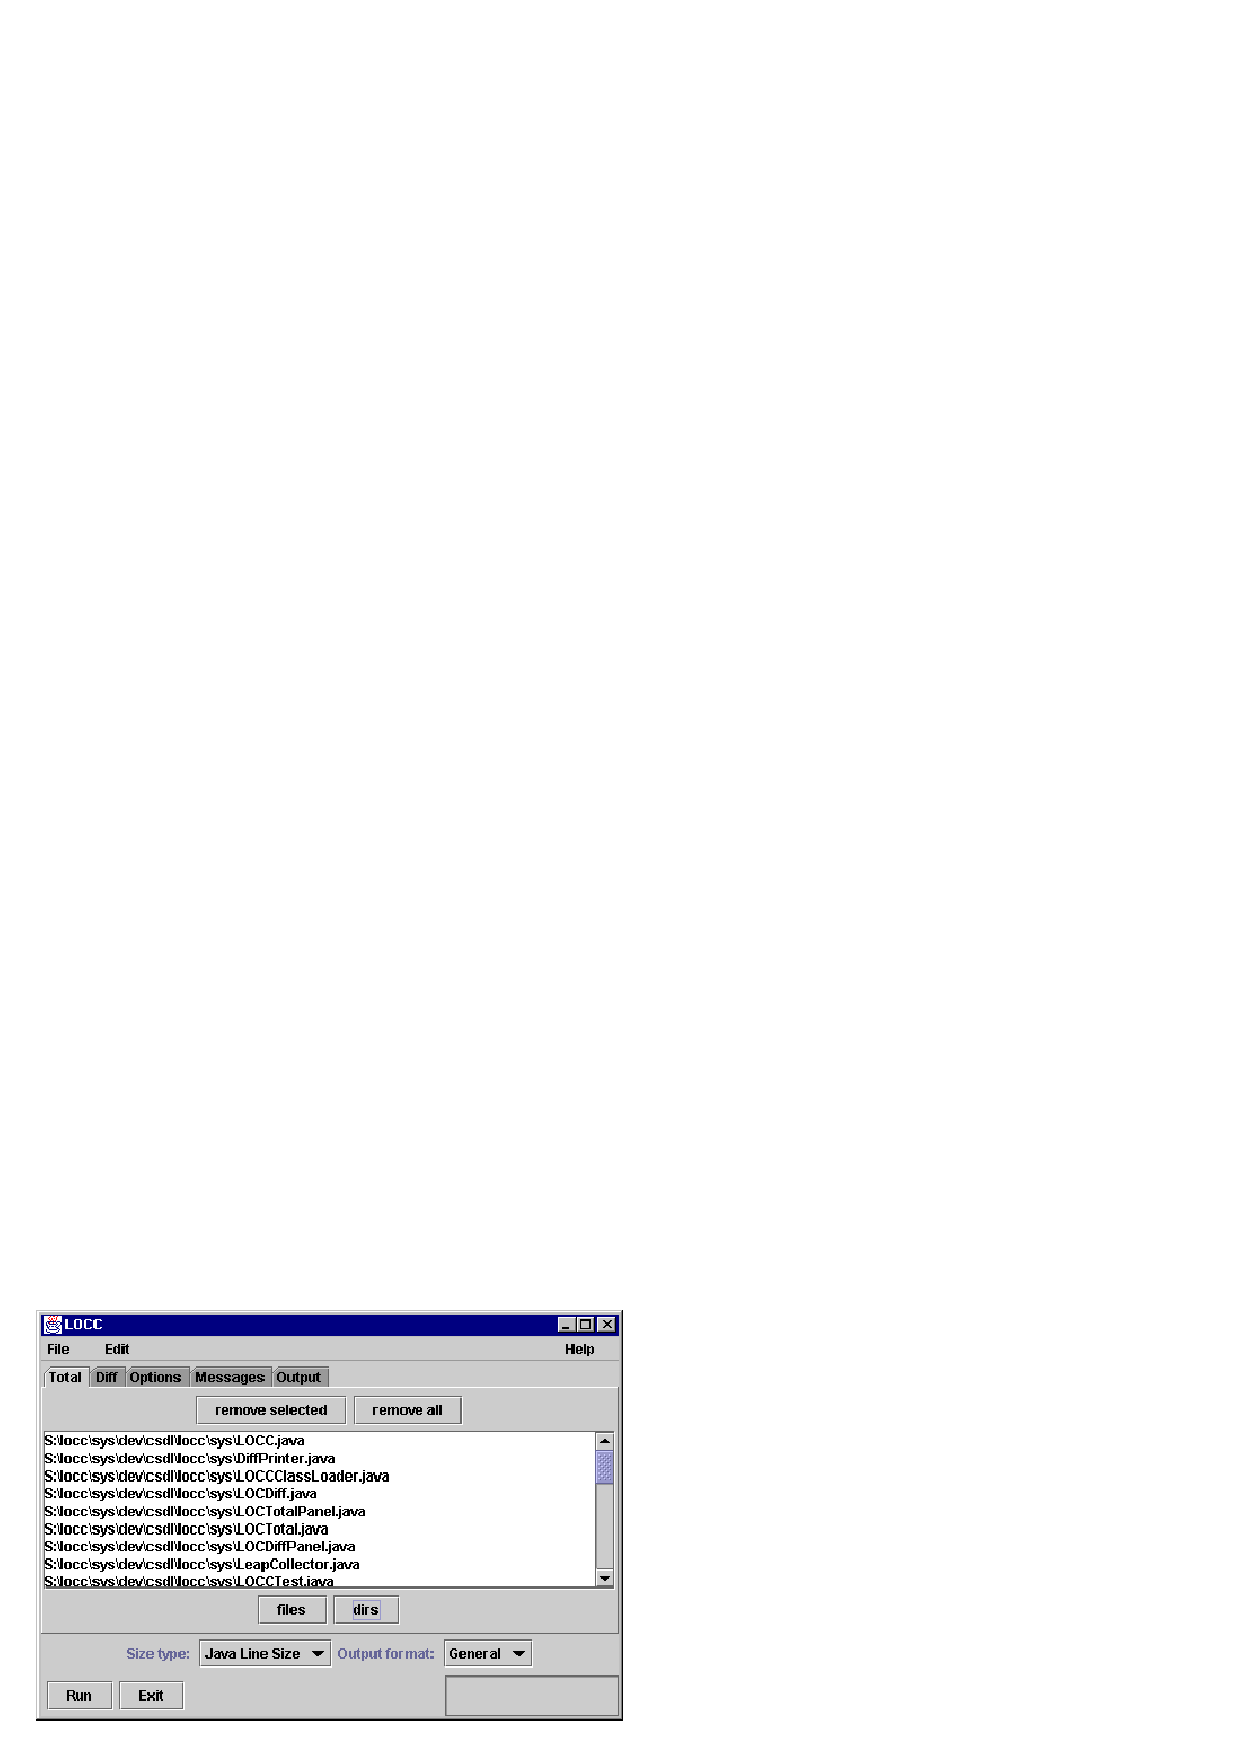
\includegraphics[angle=-90,width=4in]{figs/total-panel.epsi}
  \caption{LOCC's graphical interface}
  \label{fig:total-panel1}
\end{figure}

LOCC is currently being used both in the Collaborative Software Development
Laboratory at the University of Hawai`i, and in a graduate software engineering
class.  The initial version of LOCC was deployed in July, 1999 in the CSDL.
It has since gone through two major revisions and numerous minor revisions.
LOCC has been used to count over 50,000 lines of
Java source code.  Figure \ref{fig:total-panel1} shows a screen shot of an LOCC
session.

LOCC has been evaluated in three ways: through its use in measuring
the size of Java programs; through an online survey of current LOCC
users; and through a retrospective look at the process of extending
LOCC to include additional size metrics.  The results of the evaluation
indicate that LOCC provides a useful measurement tool, and that current
users of LOCC feel that it has assisted them in the collection of their
software process data.

The name ``LOCC'' was originally an acronym expanding to ``Lines of
Code Counter''.  This has become a misnomer, since LOCC is in no way
limited to counting lines of code.  But, inertia being what it is,
the name has stuck. 

\section{Contributions}

LOCC makes a number of important contributions to the software engineering
community: 

\begin{itemize}
  \item A Java program, portable to any platform on which Java is
    supported, which assists in the collection of program size data
  \item A graphical interface for ease of use and a flexible command line
    interface for use within scripts
  \item A method of collecting numerous size metrics together for cross
    checking or counting different types of work products
  \item A specific proposal for counting Java source code which considers
    program structure and iterative development
\end{itemize}
    
The fact that LOCC is implemented as a Java program means that it is
instantly portable to the numerous platforms which support Java.  The idea
that one tool should support more than one size metric is, as far as I
know, novel.  LOCC provides an environment conducive to experimentation
with size metrics.  Changes can be made to existing metrics, or new metrics 
installed, with a minimal expenditure of effort.  Of course, the problem of 
``which size metric should I use'' is still difficult.  LOCC can assist by
allowing a developer to use multiple metrics, deferring the decision on
which is most appropriate until enough data has been collected to make a
rational judgment.


\section{Outline of the thesis}

The thesis will cover the following topics.  Chapter \ref{chap:size} will
discuss size measurement in general.  Some reasons why program size
measurement is interesting will be discussed, and several size measures
will be introduced and described.  Chapter \ref{chap:op} will describe the
operation of LOCC. Chapter \ref{chap:arch} will describe the architecture
and implementation of LOCC.  Chapter \ref{chap:add} will examine the steps
needed to extend LOCC with new size metrics, and will go through a simple
example.  Chapter \ref{chap:eval} will give an evaluation of LOCC based on
its use in a graduate software engineering class.  Finally, Chapter
\ref{chap:future} will briefly describe some possible future directions for
LOCC.



